\documentclass{ximera}

%\usepackage{todonotes}
%\usepackage{mathtools} %% Required for wide table Curl and Greens
%\usepackage{cuted} %% Required for wide table Curl and Greens
\newcommand{\todo}{}

\usepackage{esint} % for \oiint
\ifxake%%https://math.meta.stackexchange.com/questions/9973/how-do-you-render-a-closed-surface-double-integral
\renewcommand{\oiint}{{\large\bigcirc}\kern-1.56em\iint}
\fi


\graphicspath{
  {./}
  {ximeraTutorial/}
  {basicPhilosophy/}
  {functionsOfSeveralVariables/}
  {normalVectors/}
  {lagrangeMultipliers/}
  {vectorFields/}
  {greensTheorem/}
  {shapeOfThingsToCome/}
  {dotProducts/}
  {partialDerivativesAndTheGradientVector/}
  {../productAndQuotientRules/exercises/}
  {../normalVectors/exercisesParametricPlots/}
  {../continuityOfFunctionsOfSeveralVariables/exercises/}
  {../partialDerivativesAndTheGradientVector/exercises/}
  {../directionalDerivativeAndChainRule/exercises/}
  {../commonCoordinates/exercisesCylindricalCoordinates/}
  {../commonCoordinates/exercisesSphericalCoordinates/}
  {../greensTheorem/exercisesCurlAndLineIntegrals/}
  {../greensTheorem/exercisesDivergenceAndLineIntegrals/}
  {../shapeOfThingsToCome/exercisesDivergenceTheorem/}
  {../greensTheorem/}
  {../shapeOfThingsToCome/}
  {../separableDifferentialEquations/exercises/}
  {vectorFields/}
}

\newcommand{\mooculus}{\textsf{\textbf{MOOC}\textnormal{\textsf{ULUS}}}}

\usepackage{tkz-euclide}\usepackage{tikz}
\usepackage{tikz-cd}
\usetikzlibrary{arrows}
\tikzset{>=stealth,commutative diagrams/.cd,
  arrow style=tikz,diagrams={>=stealth}} %% cool arrow head
\tikzset{shorten <>/.style={ shorten >=#1, shorten <=#1 } } %% allows shorter vectors

\usetikzlibrary{backgrounds} %% for boxes around graphs
\usetikzlibrary{shapes,positioning}  %% Clouds and stars
\usetikzlibrary{matrix} %% for matrix
\usepgfplotslibrary{polar} %% for polar plots
\usepgfplotslibrary{fillbetween} %% to shade area between curves in TikZ
\usetkzobj{all}
\usepackage[makeroom]{cancel} %% for strike outs
%\usepackage{mathtools} %% for pretty underbrace % Breaks Ximera
%\usepackage{multicol}
\usepackage{pgffor} %% required for integral for loops



%% http://tex.stackexchange.com/questions/66490/drawing-a-tikz-arc-specifying-the-center
%% Draws beach ball
\tikzset{pics/carc/.style args={#1:#2:#3}{code={\draw[pic actions] (#1:#3) arc(#1:#2:#3);}}}



\usepackage{array}
\setlength{\extrarowheight}{+.1cm}
\newdimen\digitwidth
\settowidth\digitwidth{9}
\def\divrule#1#2{
\noalign{\moveright#1\digitwidth
\vbox{\hrule width#2\digitwidth}}}





\newcommand{\RR}{\mathbb R}
\newcommand{\R}{\mathbb R}
\newcommand{\N}{\mathbb N}
\newcommand{\Z}{\mathbb Z}

\newcommand{\sagemath}{\textsf{SageMath}}


%\renewcommand{\d}{\,d\!}
\renewcommand{\d}{\mathop{}\!d}
\newcommand{\dd}[2][]{\frac{\d #1}{\d #2}}
\newcommand{\pp}[2][]{\frac{\partial #1}{\partial #2}}
\renewcommand{\l}{\ell}
\newcommand{\ddx}{\frac{d}{\d x}}

\newcommand{\zeroOverZero}{\ensuremath{\boldsymbol{\tfrac{0}{0}}}}
\newcommand{\inftyOverInfty}{\ensuremath{\boldsymbol{\tfrac{\infty}{\infty}}}}
\newcommand{\zeroOverInfty}{\ensuremath{\boldsymbol{\tfrac{0}{\infty}}}}
\newcommand{\zeroTimesInfty}{\ensuremath{\small\boldsymbol{0\cdot \infty}}}
\newcommand{\inftyMinusInfty}{\ensuremath{\small\boldsymbol{\infty - \infty}}}
\newcommand{\oneToInfty}{\ensuremath{\boldsymbol{1^\infty}}}
\newcommand{\zeroToZero}{\ensuremath{\boldsymbol{0^0}}}
\newcommand{\inftyToZero}{\ensuremath{\boldsymbol{\infty^0}}}



\newcommand{\numOverZero}{\ensuremath{\boldsymbol{\tfrac{\#}{0}}}}
\newcommand{\dfn}{\textbf}
%\newcommand{\unit}{\,\mathrm}
\newcommand{\unit}{\mathop{}\!\mathrm}
\newcommand{\eval}[1]{\bigg[ #1 \bigg]}
\newcommand{\seq}[1]{\left( #1 \right)}
\renewcommand{\epsilon}{\varepsilon}
\renewcommand{\phi}{\varphi}


\renewcommand{\iff}{\Leftrightarrow}

\DeclareMathOperator{\arccot}{arccot}
\DeclareMathOperator{\arcsec}{arcsec}
\DeclareMathOperator{\arccsc}{arccsc}
\DeclareMathOperator{\si}{Si}
\DeclareMathOperator{\scal}{scal}
\DeclareMathOperator{\sign}{sign}


%% \newcommand{\tightoverset}[2]{% for arrow vec
%%   \mathop{#2}\limits^{\vbox to -.5ex{\kern-0.75ex\hbox{$#1$}\vss}}}
\newcommand{\arrowvec}[1]{{\overset{\rightharpoonup}{#1}}}
%\renewcommand{\vec}[1]{\arrowvec{\mathbf{#1}}}
\renewcommand{\vec}[1]{{\overset{\boldsymbol{\rightharpoonup}}{\mathbf{#1}}}\hspace{0in}}

\newcommand{\point}[1]{\left(#1\right)} %this allows \vector{ to be changed to \vector{ with a quick find and replace
\newcommand{\pt}[1]{\mathbf{#1}} %this allows \vec{ to be changed to \vec{ with a quick find and replace
\newcommand{\Lim}[2]{\lim_{\point{#1} \to \point{#2}}} %Bart, I changed this to point since I want to use it.  It runs through both of the exercise and exerciseE files in limits section, which is why it was in each document to start with.

\DeclareMathOperator{\proj}{\mathbf{proj}}
\newcommand{\veci}{{\boldsymbol{\hat{\imath}}}}
\newcommand{\vecj}{{\boldsymbol{\hat{\jmath}}}}
\newcommand{\veck}{{\boldsymbol{\hat{k}}}}
\newcommand{\vecl}{\vec{\boldsymbol{\l}}}
\newcommand{\uvec}[1]{\mathbf{\hat{#1}}}
\newcommand{\utan}{\mathbf{\hat{t}}}
\newcommand{\unormal}{\mathbf{\hat{n}}}
\newcommand{\ubinormal}{\mathbf{\hat{b}}}

\newcommand{\dotp}{\bullet}
\newcommand{\cross}{\boldsymbol\times}
\newcommand{\grad}{\boldsymbol\nabla}
\newcommand{\divergence}{\grad\dotp}
\newcommand{\curl}{\grad\cross}
%\DeclareMathOperator{\divergence}{divergence}
%\DeclareMathOperator{\curl}[1]{\grad\cross #1}
\newcommand{\lto}{\mathop{\longrightarrow\,}\limits}

\renewcommand{\bar}{\overline}

\colorlet{textColor}{black}
\colorlet{background}{white}
\colorlet{penColor}{blue!50!black} % Color of a curve in a plot
\colorlet{penColor2}{red!50!black}% Color of a curve in a plot
\colorlet{penColor3}{red!50!blue} % Color of a curve in a plot
\colorlet{penColor4}{green!50!black} % Color of a curve in a plot
\colorlet{penColor5}{orange!80!black} % Color of a curve in a plot
\colorlet{penColor6}{yellow!70!black} % Color of a curve in a plot
\colorlet{fill1}{penColor!20} % Color of fill in a plot
\colorlet{fill2}{penColor2!20} % Color of fill in a plot
\colorlet{fillp}{fill1} % Color of positive area
\colorlet{filln}{penColor2!20} % Color of negative area
\colorlet{fill3}{penColor3!20} % Fill
\colorlet{fill4}{penColor4!20} % Fill
\colorlet{fill5}{penColor5!20} % Fill
\colorlet{gridColor}{gray!50} % Color of grid in a plot

\newcommand{\surfaceColor}{violet}
\newcommand{\surfaceColorTwo}{redyellow}
\newcommand{\sliceColor}{greenyellow}




\pgfmathdeclarefunction{gauss}{2}{% gives gaussian
  \pgfmathparse{1/(#2*sqrt(2*pi))*exp(-((x-#1)^2)/(2*#2^2))}%
}


%%%%%%%%%%%%%
%% Vectors
%%%%%%%%%%%%%

%% Simple horiz vectors
\renewcommand{\vector}[1]{\left\langle #1\right\rangle}


%% %% Complex Horiz Vectors with angle brackets
%% \makeatletter
%% \renewcommand{\vector}[2][ , ]{\left\langle%
%%   \def\nextitem{\def\nextitem{#1}}%
%%   \@for \el:=#2\do{\nextitem\el}\right\rangle%
%% }
%% \makeatother

%% %% Vertical Vectors
%% \def\vector#1{\begin{bmatrix}\vecListA#1,,\end{bmatrix}}
%% \def\vecListA#1,{\if,#1,\else #1\cr \expandafter \vecListA \fi}

%%%%%%%%%%%%%
%% End of vectors
%%%%%%%%%%%%%

%\newcommand{\fullwidth}{}
%\newcommand{\normalwidth}{}



%% makes a snazzy t-chart for evaluating functions
%\newenvironment{tchart}{\rowcolors{2}{}{background!90!textColor}\array}{\endarray}

%%This is to help with formatting on future title pages.
\newenvironment{sectionOutcomes}{}{}



%% Flowchart stuff
%\tikzstyle{startstop} = [rectangle, rounded corners, minimum width=3cm, minimum height=1cm,text centered, draw=black]
%\tikzstyle{question} = [rectangle, minimum width=3cm, minimum height=1cm, text centered, draw=black]
%\tikzstyle{decision} = [trapezium, trapezium left angle=70, trapezium right angle=110, minimum width=3cm, minimum height=1cm, text centered, draw=black]
%\tikzstyle{question} = [rectangle, rounded corners, minimum width=3cm, minimum height=1cm,text centered, draw=black]
%\tikzstyle{process} = [rectangle, minimum width=3cm, minimum height=1cm, text centered, draw=black]
%\tikzstyle{decision} = [trapezium, trapezium left angle=70, trapezium right angle=110, minimum width=3cm, minimum height=1cm, text centered, draw=black]


\outcome{Define a vector field.}
\outcome{Identify radial vector fields.}
\outcome{Identify gradient vector fields.}
\outcome{Find potential functions for gradient fields.}

\title[Dig-In:]{Vector fields}

\begin{document}
\begin{abstract}
  We introduce the idea of a vector at every point in space. 
\end{abstract}
\maketitle

\section{A review of functions}

When we started on our journey exploring calculus, we investigated
functions:
\[
f:\R \to \R
\]
Typically, we interpert these functions as being curves in the
$(x,y)$-plane:
\begin{image}
\begin{tikzpicture}
	\begin{axis}[
            xmin=-3.25,xmax=3.25,ymin=-1.5,ymax=1.5,
            axis lines=center,
            xtick={-6.28, -4.71, -3.14, -1.57, 0, 1.57, 3.142, 4.71, 6.28},
            xticklabels={$-2\pi$,$-3\pi/2$,$-\pi$, $-\pi/2$, $0$, $\pi/2$, $\pi$, $3\pi/2$, $2\pi$},
            ytick={-1,1},
            %ticks=none,
            width=3in,
            height=3in,
            unit vector ratio*=1 1 1,
            xlabel=$x$, ylabel=$y$,
            every axis y label/.style={at=(current axis.above origin),anchor=south},
            every axis x label/.style={at=(current axis.right of origin),anchor=west},
          ]        
          \addplot [very thick, penColor, samples=100,smooth, domain=(-3.25:3.25)] {sin(deg(x))};
        \end{axis}
\end{tikzpicture}
%% \caption{The function $\sin(\theta)$ takes on all values between $-1$
%%   and $1$ exactly once on the interval $[-\pi/2,\pi/2]$. If we
%%   restrict $\sin(\theta)$ to this interval, then this restricted
%%   function has an inverse.}
%% \label{figure:sin-restricted}
%% \end{figure*}
\end{image}
We've also studied vector valued functions:
\[
\vec{f}:\R \to \R^n
\]
We can interpert these functions as parametric curves in space:
\begin{image}
    \begin{tikzpicture}
      \begin{axis}%
        [tick label style={font=\scriptsize},axis on top,
	  axis lines=center,
	  view={155}{10},no markers,
	  ymin=-1.1,ymax=1.1,
	  xmin=-7,xmax=7,
	  zmin=-1.1, zmax=1.1,
	  every axis x label/.style={at={(axis cs:\pgfkeysvalueof{/pgfplots/xmax},0,0)},xshift=-3pt,yshift=-3pt},
	  xlabel={\scriptsize $x$},
	  every axis y label/.style={at={(axis cs:0,\pgfkeysvalueof{/pgfplots/ymax},0)},xshift=5pt,yshift=-2pt},
	  ylabel={\scriptsize $y$},
	  every axis z label/.style={at={(axis cs:0,0,\pgfkeysvalueof{/pgfplots/zmax})},xshift=0pt,yshift=4pt},
	  zlabel={\scriptsize $z$}
	]
        \draw[thick,->,penColor!50!white] (axis cs: 0,0,0)--(axis cs: {-4},{sin(deg(-4))},{cos(deg(-4))});
        \draw[thick,->,penColor!50!white] (axis cs: 0,0,0)--(axis cs: {-3},{sin(deg(-3))},{cos(deg(-3))});
        \draw[thick,->,penColor!50!white] (axis cs: 0,0,0)--(axis cs: {-2},{sin(deg(-2))},{cos(deg(-2))});
        \draw[thick,->,penColor!50!white] (axis cs: 0,0,0)--(axis cs: {-1},{sin(deg(-1))},{cos(deg(-1))});
        \draw[thick,->,penColor!50!white] (axis cs: 0,0,0)--(axis cs: {0},{sin(deg(0))},{cos(deg(0))});
        \draw[thick,->,penColor!50!white] (axis cs: 0,0,0)--(axis cs: {1},{sin(deg(1))},{cos(deg(1))});
        \draw[thick,->,penColor!50!white] (axis cs: 0,0,0)--(axis cs: {2},{sin(deg(2))},{cos(deg(2))});
        \draw[thick,->,penColor!50!white] (axis cs: 0,0,0)--(axis cs: {3},{sin(deg(3))},{cos(deg(3))});
        \draw[thick,->,penColor!50!white] (axis cs: 0,0,0)--(axis cs: {4},{sin(deg(4))},{cos(deg(4))});
        \addplot3+[very thick, penColor, smooth,samples=200,samples y=0,domain=-12:12] ({x},{sin(deg(x))},{cos(deg(x)});
      \end{axis}
    \end{tikzpicture}
    \end{image}
We've studied functions of several variables
\[
F:\R^n \to \R
\]
We can interpert these functions as surfaces in $\R^{n+1}$,
\begin{image}
  \begin{tikzpicture}
    \begin{axis}%
      [width=175pt,tick label style={font=\scriptsize},axis on top,
	axis lines=center,
	view={155}{30},
	name=myplot,
	xtick=\empty,
	ytick=\empty,
	ztick=\empty,
	ymin=-1.2,ymax=1.2,
	xmin=-1.2,xmax=1.2,
	zmin=-1.2, zmax=1.2,
	every axis x label/.style={at={(axis cs:\pgfkeysvalueof{/pgfplots/xmax},0,0)},xshift=-3pt,yshift=-3pt},
	xlabel={\scriptsize $x$},
	every axis y label/.style={at={(axis cs:0,\pgfkeysvalueof{/pgfplots/ymax},0)},xshift=5pt,yshift=-2pt},
	ylabel={\scriptsize $y$},
	every axis z label/.style={at={(axis cs:0,0,\pgfkeysvalueof{/pgfplots/zmax})},xshift=0pt,yshift=4pt},
	zlabel={\scriptsize $z$},
        colormap/cool
      ]

      \addplot3[domain=-1:1,smooth,y domain=-1:1,mesh,samples=20,samples y=25,very thin,z buffer=sort] ({x},{y},{x^2-y^2});
    \end{axis}
  \end{tikzpicture}
\end{image}


Now we study vector-valued functions of several variables
\[
\vec{F}:\R^n\to R^n
\]
and we intererpert these as \textit{vector fields}, meaning for each
point in the $(x,y)$-plane we have a vector.
\begin{image}
  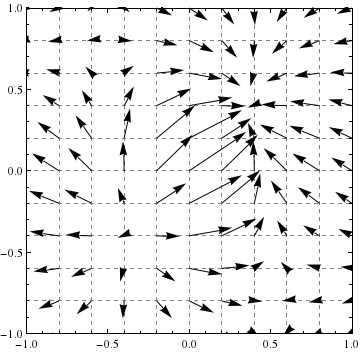
\includegraphics{egField.png}
\end{image}


Let's be explicit
\begin{definition}
  A \dfn{vector field} in $\R^n$ is a function
  \[
  \vec{F}: \R^n\to\R^n
  \]
  where for every point in the domain, we assign a vector to the range. 
\end{definition}

\begin{question}
  Consider the following table describing a vector field $\vec{F}$:
  \begin{image}
    \begin{tikzpicture}[x=.75cm,y=.5cm]
      \draw (0,0) grid [step=1] (1,4);
      \draw (3,4) -- (3,0);
      \draw (5,4) -- (5,0);
      \draw (7,4) -- (7,0);
      \draw (9,4) -- (9,0);
      
      \draw (0,0) -- (9,0);
      \draw (0,1) -- (9,1);
      \draw (0,2) -- (9,2);
      \draw (0,3) -- (9,3);
      \draw (0,4) -- (9,4);
      
      \draw[ultra thick] (0,1)--(9,1);
      \draw[ultra thick] (1,4)--(1,0);
      
      \draw (0,0) -- (1,1);
      %\node at (.9,.9) [below left,inner sep=1pt] {\small$y$};
      %\node at (0.1,.1) [above right,inner sep=1pt] {\small$x$};
      \node at (.1,.9) [below right,inner sep=1pt] {\small$y$};
      \node at (0.9,.1) [above left,inner sep=1pt] {\small$x$};


      %% x-values
      \node at (2,.5) {$1$};
      \node at (4,.5) {$2$};
      \node at (6,.5) {$3$};
      \node at (8,.5) {$4$};

      %% y-values
      \node at (0.5,1.5) {$5$};
      \node at (0.5,2.5) {$6$};
      \node at (0.5,3.5) {$7$};
      
      
      %% vectors
      %% bottom row
      \node at (2,1.5) {$\veci+2\vecj$};
      \node at (4,1.5) {$-3\vecj$};
      \node at (6,1.5) {$2\vecj$};
      \node at (8,1.5) {$2\veci+4\vecj$};
      
      %% second row
      \node at (2,2.5) {$3\vecj$};
      \node at (4,2.5) {$\vec{0}$};
      \node at (6,2.5) {$2\veci-3\vecj$};
      \node at (8,2.5) {$\veci-2\vecj$};
      
      %% third row
      \node at (2,3.5) {$\veci-\vecj$};
      \node at (4,3.5) {$-2\vecj$};
      \node at (6,3.5) {$-2\veci-2\vecj$};
      \node at (8,3.5) {$\veci$};

    \end{tikzpicture}
  \end{image}
  What is $\vec{F}(1,7)$?
  \begin{prompt}
    \[
    \vec{F}(1,7) = \vector{\answer{1},\answer{-1}}
    \]
  \end{prompt}
  \begin{question}
    What is $\vec{F}(3,5)$?
    \begin{prompt}
      \[
      \vec{F}(3,5) = \vector{\answer{0},\answer{2}}
      \]
    \end{prompt}
    \begin{question}
      What is $\vec{F}(2,6)$?
      \begin{prompt}
        \[
        \vec{F}(2,6) = \vector{\answer{0},\answer{0}}
        \]
      \end{prompt}
    \end{question}
  \end{question}
\end{question}

\begin{question}
  Consider the following vector field:
  \begin{image}
    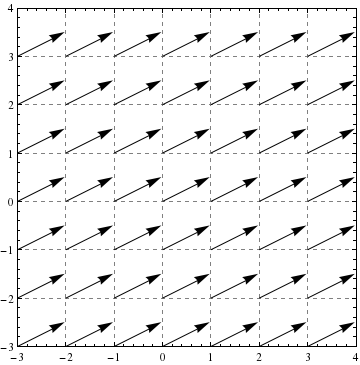
\includegraphics{constField.png}
  \end{image}
  Which expression is best described by this vector field?
  \begin{multipleChoice}
    \choice{$\vec{F}(x,y)=\vector{x,y/2}$}
    \choice{$\vec{F}(x,y)=1/2$}
    \choice{$\vec{F}(x,y)=x+y/2$}
    \choice[correct]{$\vec{F}(x,y)=\vector{1,1/2}$}
  \end{multipleChoice}
  \begin{feedback}[correct]
    Note, $\grad(x+y/2) = \vector{1,1/2}$.
  \end{feedback}
\end{question}



Now we give you a small sampling of some important vector fields.


\section{Radial fields}

Let's see some examples of radial vector fields:
\begin{example}
  Here we see
  \[
  \vec{F}(x,y) = \vector{\frac{x}{\sqrt{x^2+y^2}},\frac{y}{\sqrt{x^2+y^2}}}:
  \]
  \begin{image}
    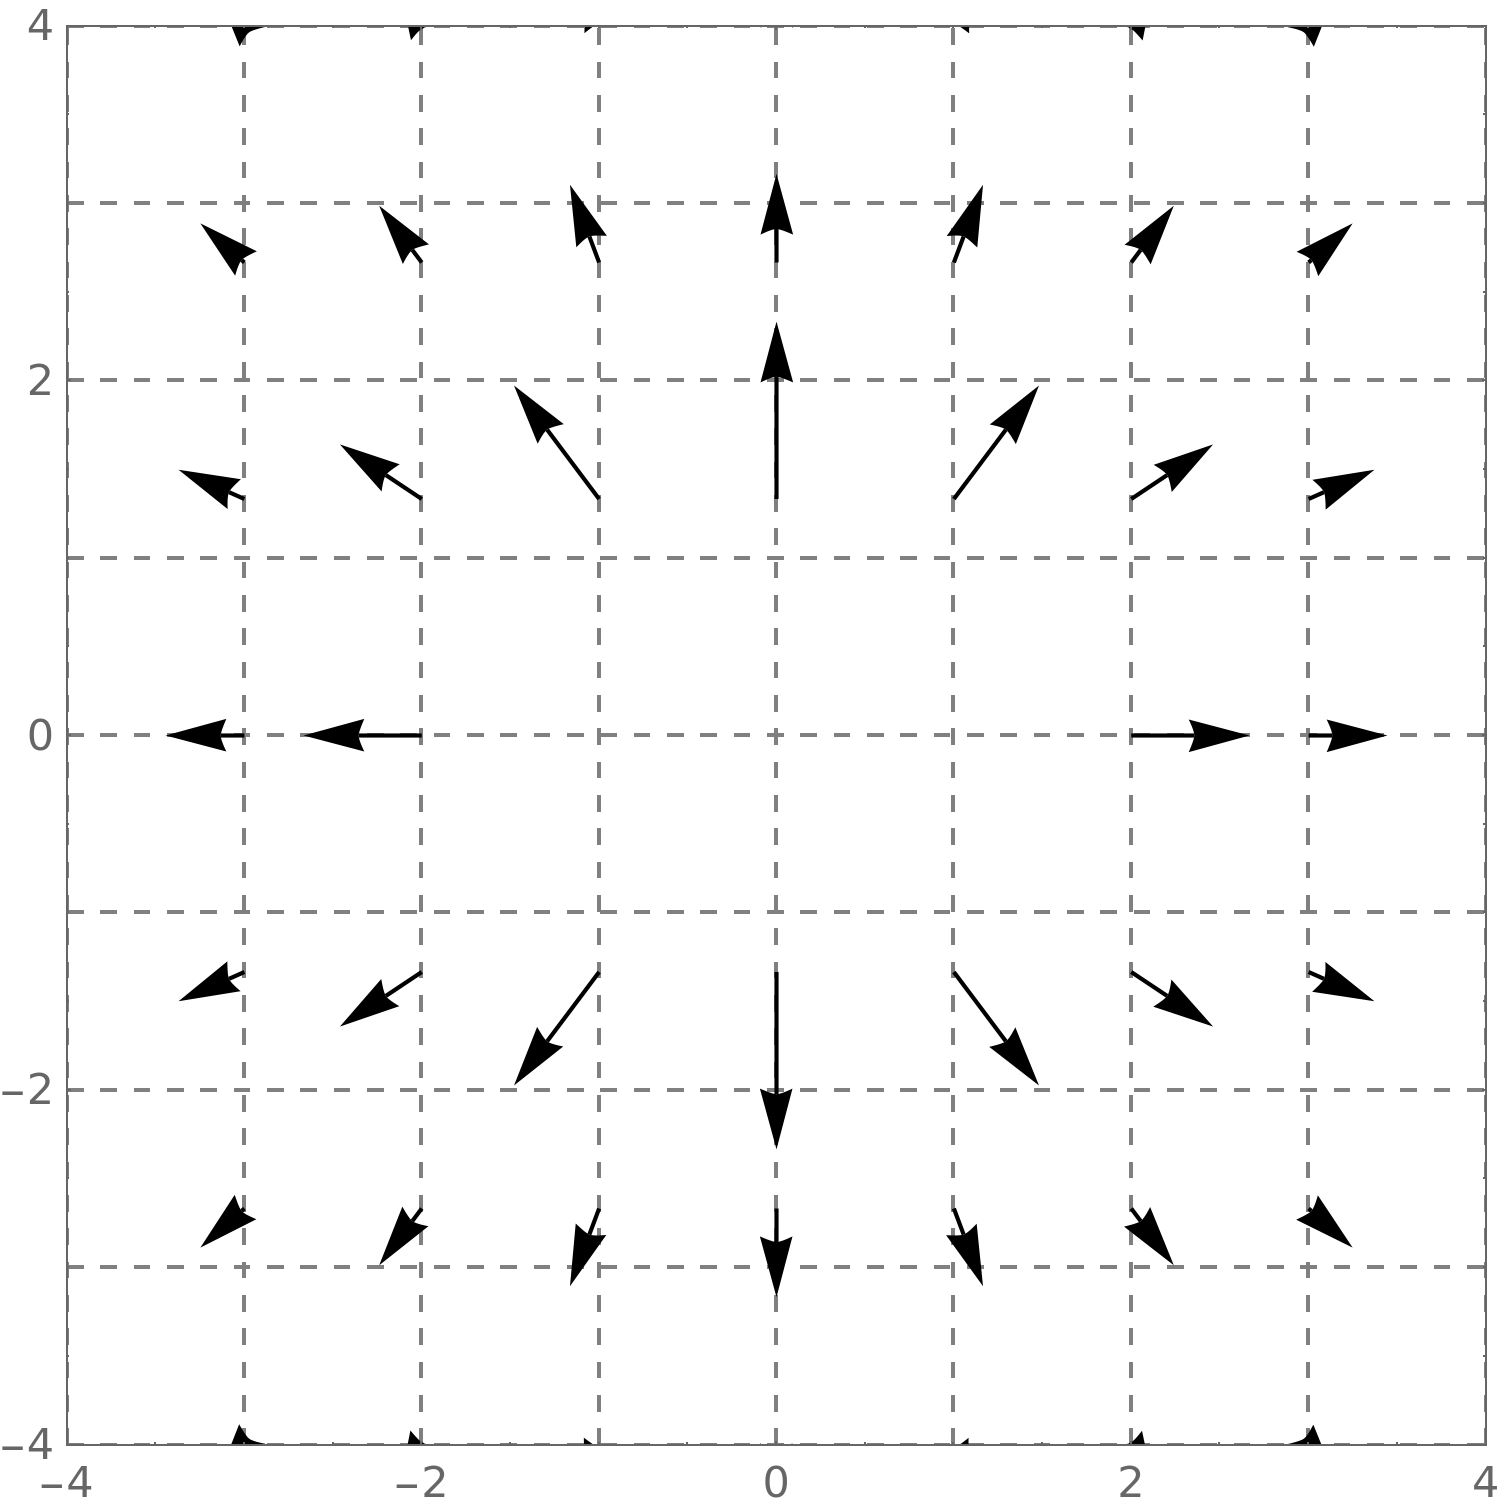
\includegraphics{radField1.png}
  \end{image}
\end{example}

\begin{example}
  Here we see
  \[
  \vec{G}(x,y) = \vector{\frac{-x}{x^2+y^2},\frac{-y}{x^2+y^2}}:
  \]
  \begin{image}
    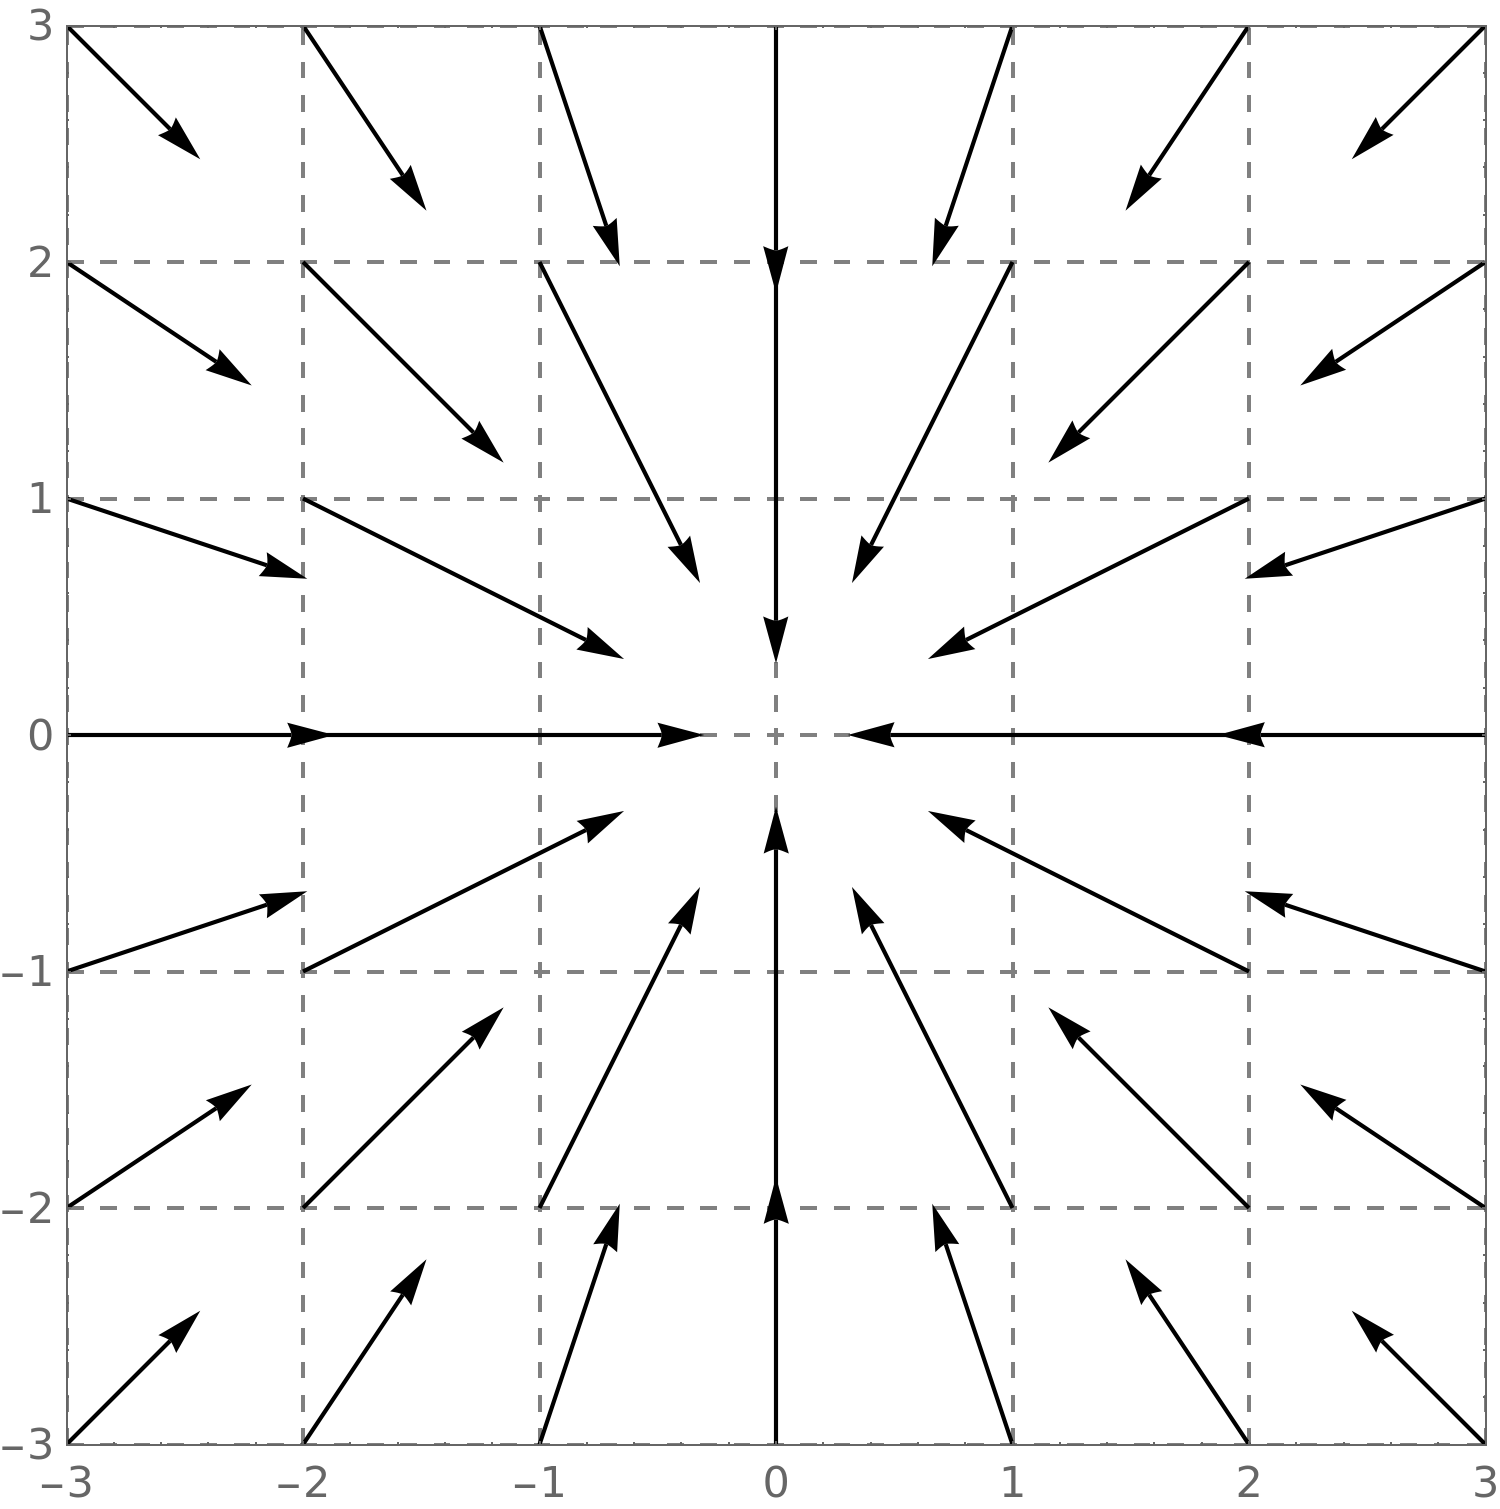
\includegraphics{radField2.png}
  \end{image}
\end{example}

\begin{example}
  Here we see
  \[
  \vec{H}(x,y,z) = \vector{\frac{x}{(x^2+y^2+z^2)^2},\frac{y}{(x^2+y^2+z^2)^2},\frac{z}{(x^2+y^2+z^2)^2}}:
  \]
  \begin{image}
    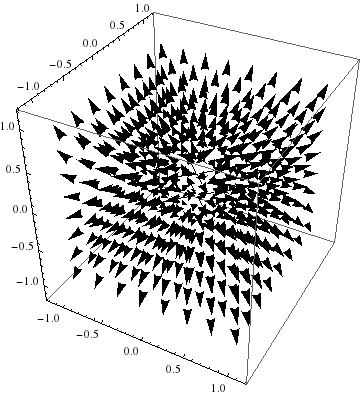
\includegraphics{radField3.png}
  \end{image}
\end{example}

Each of the vector fields above is a \textit{radial} vector field.

\begin{definition}
  A \dfn{radial vector field} is a field of the form
  $\vec{F}:\R^n\to\R^n$ where
  \[
  \vec{F}(\vec{x}) = \frac{\pm\vec{x}}{|\vec{x}|^p}
  \]
  where $p$ is a real number. 
\end{definition}

\begin{question}
  Is $\vec{F}(x,y,z) = \vector{x,y,z}$ a radial vector field?
  \begin{prompt}
    \begin{multipleChoice}
      \choice[correct]{yes}
      \choice{no}
    \end{multipleChoice}
    \begin{feedback}[correct]
      Absolutely! This vector field can be rewritten as:
      \[
      \vector{\frac{x}{(\sqrt{x^2+y^2+z^2})^p},\frac{y}{(\sqrt{x^2+y^2+z^2})^p},\frac{z}{(\sqrt{x^2+y^2+z^2})^p}}
      \]
      where $p=\answer{0}$.
    \end{feedback}
  \end{prompt}
\end{question}



\section{Rotational fields}

Vector fields can easily exhibit what looks like ``rotation'' to the
human eye.
\begin{example}
  Here we see
  \[
  \vec{F}(x,y) = \vector{-y,x}:
  \]
  \begin{image}
    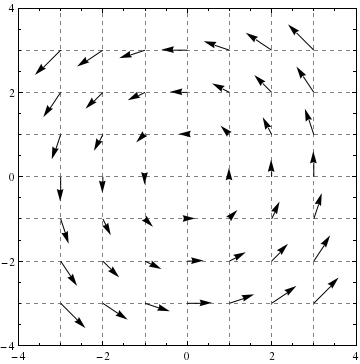
\includegraphics{rotField.png}
  \end{image}
\end{example}

\begin{example}
  Here we see
  \[
  \vec{F}(x,y) = \vector{\frac{-y}{x^2+y^2},\frac{x}{x^2+y^2}}:
  \]
  \begin{image}
    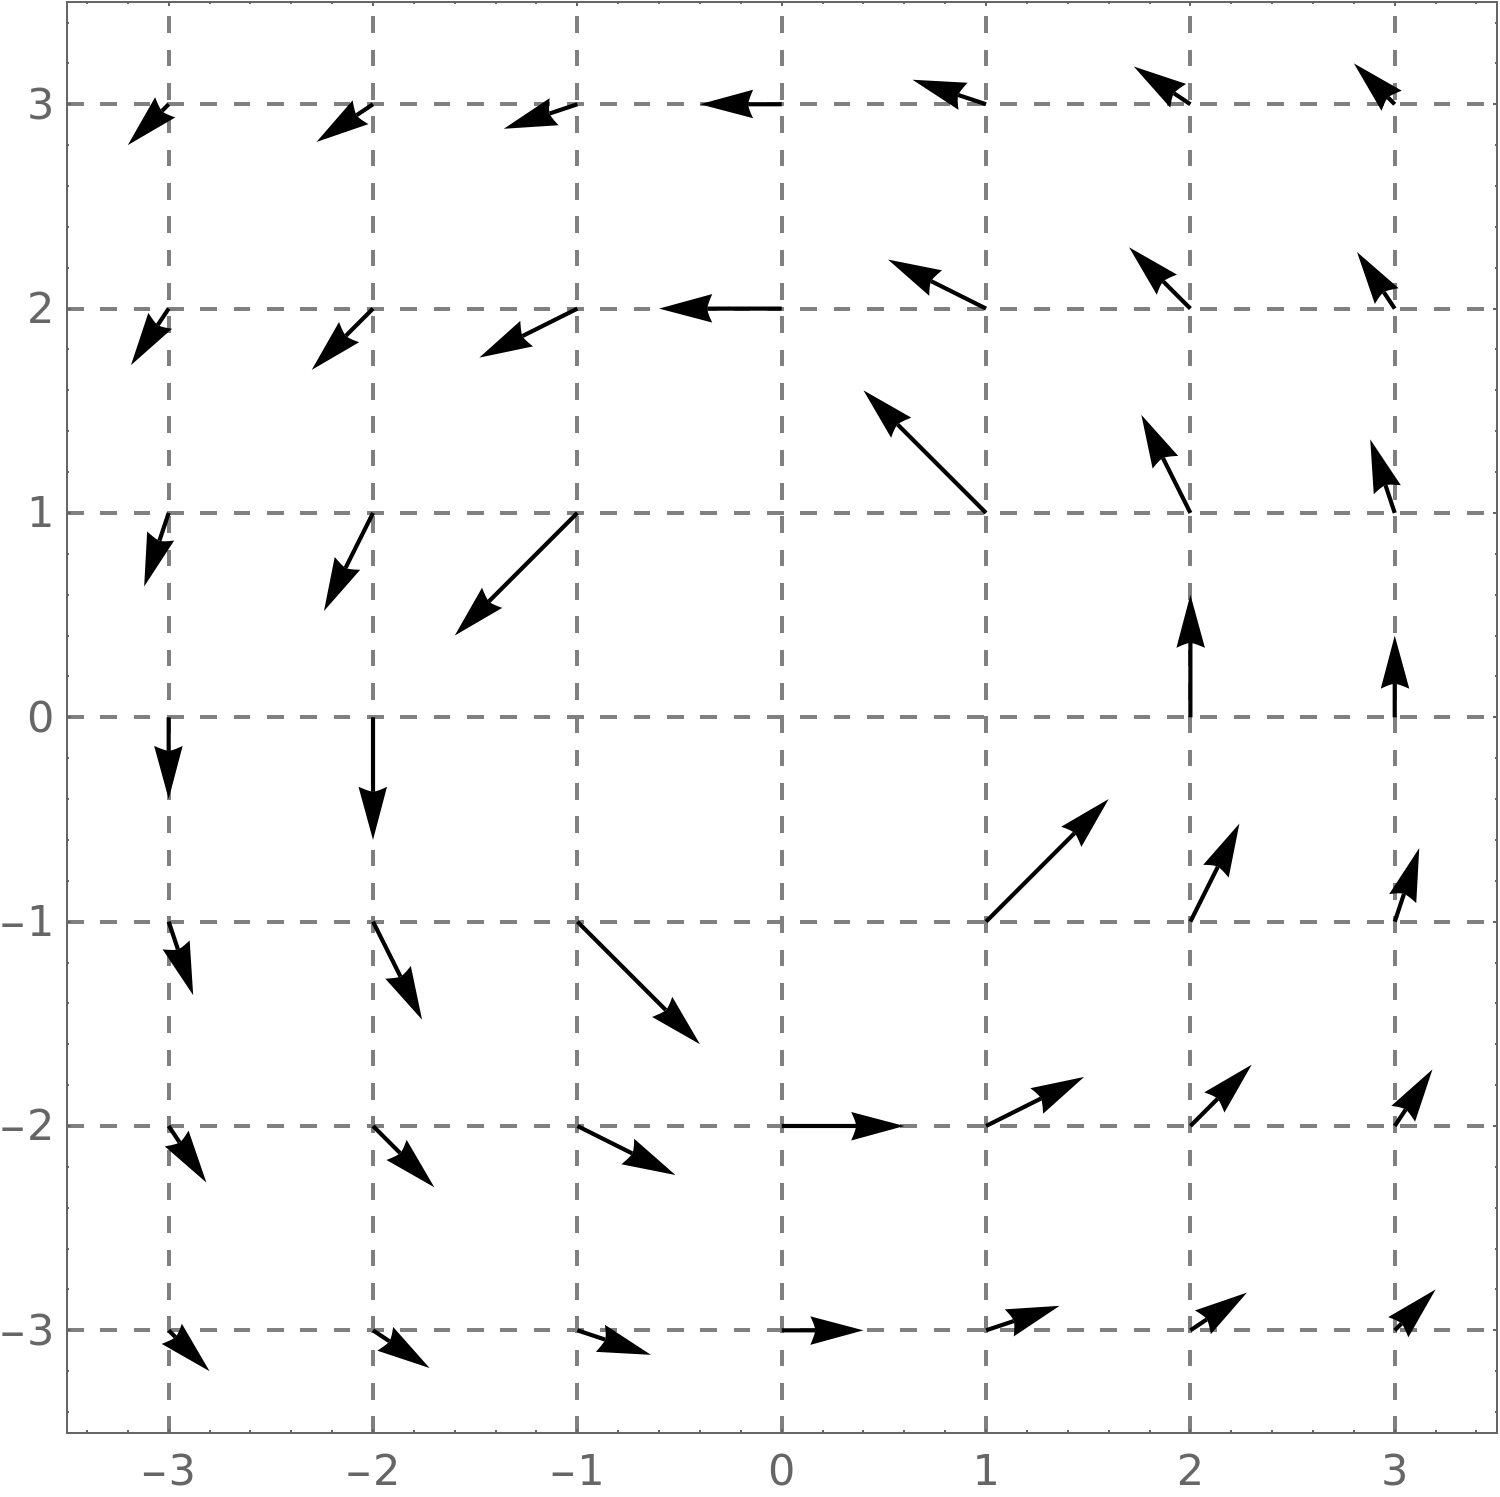
\includegraphics{rotFieldNot.png}
  \end{image}
\end{example}

At this point, we're going to give some ``spoilers.'' It turns out
that from a local perspective, meaning all points very very close each
other, only the first example exhibits ``rotation.'' While the second
example does look like it is ``rotating,'' as we will see, it does not
exhibit ``local rotation.''


\section{Gradient fields}

We're going to start with the definition.

\begin{definition}
  Consider any differentiable function $F:\R^n\to \R$.
  A \dfn{gradient field} is a vector field $\vec{G}:\R^n\to \R^n$ where
  \[
  \vec{G} = \grad F.
  \]
\end{definition}

Since we are assuming $F$ is differentiable, we are also assuming that
$\vec{G}$ is defined for all points in $\R^n$. This is important to
note, as we will see.

\begin{example}
  Consider $F(x,y) = \frac{\sin(3x)+\sin(2y)}{1+x^2+y^2}$. A plot of
  this function looks like this:
  \begin{image}
    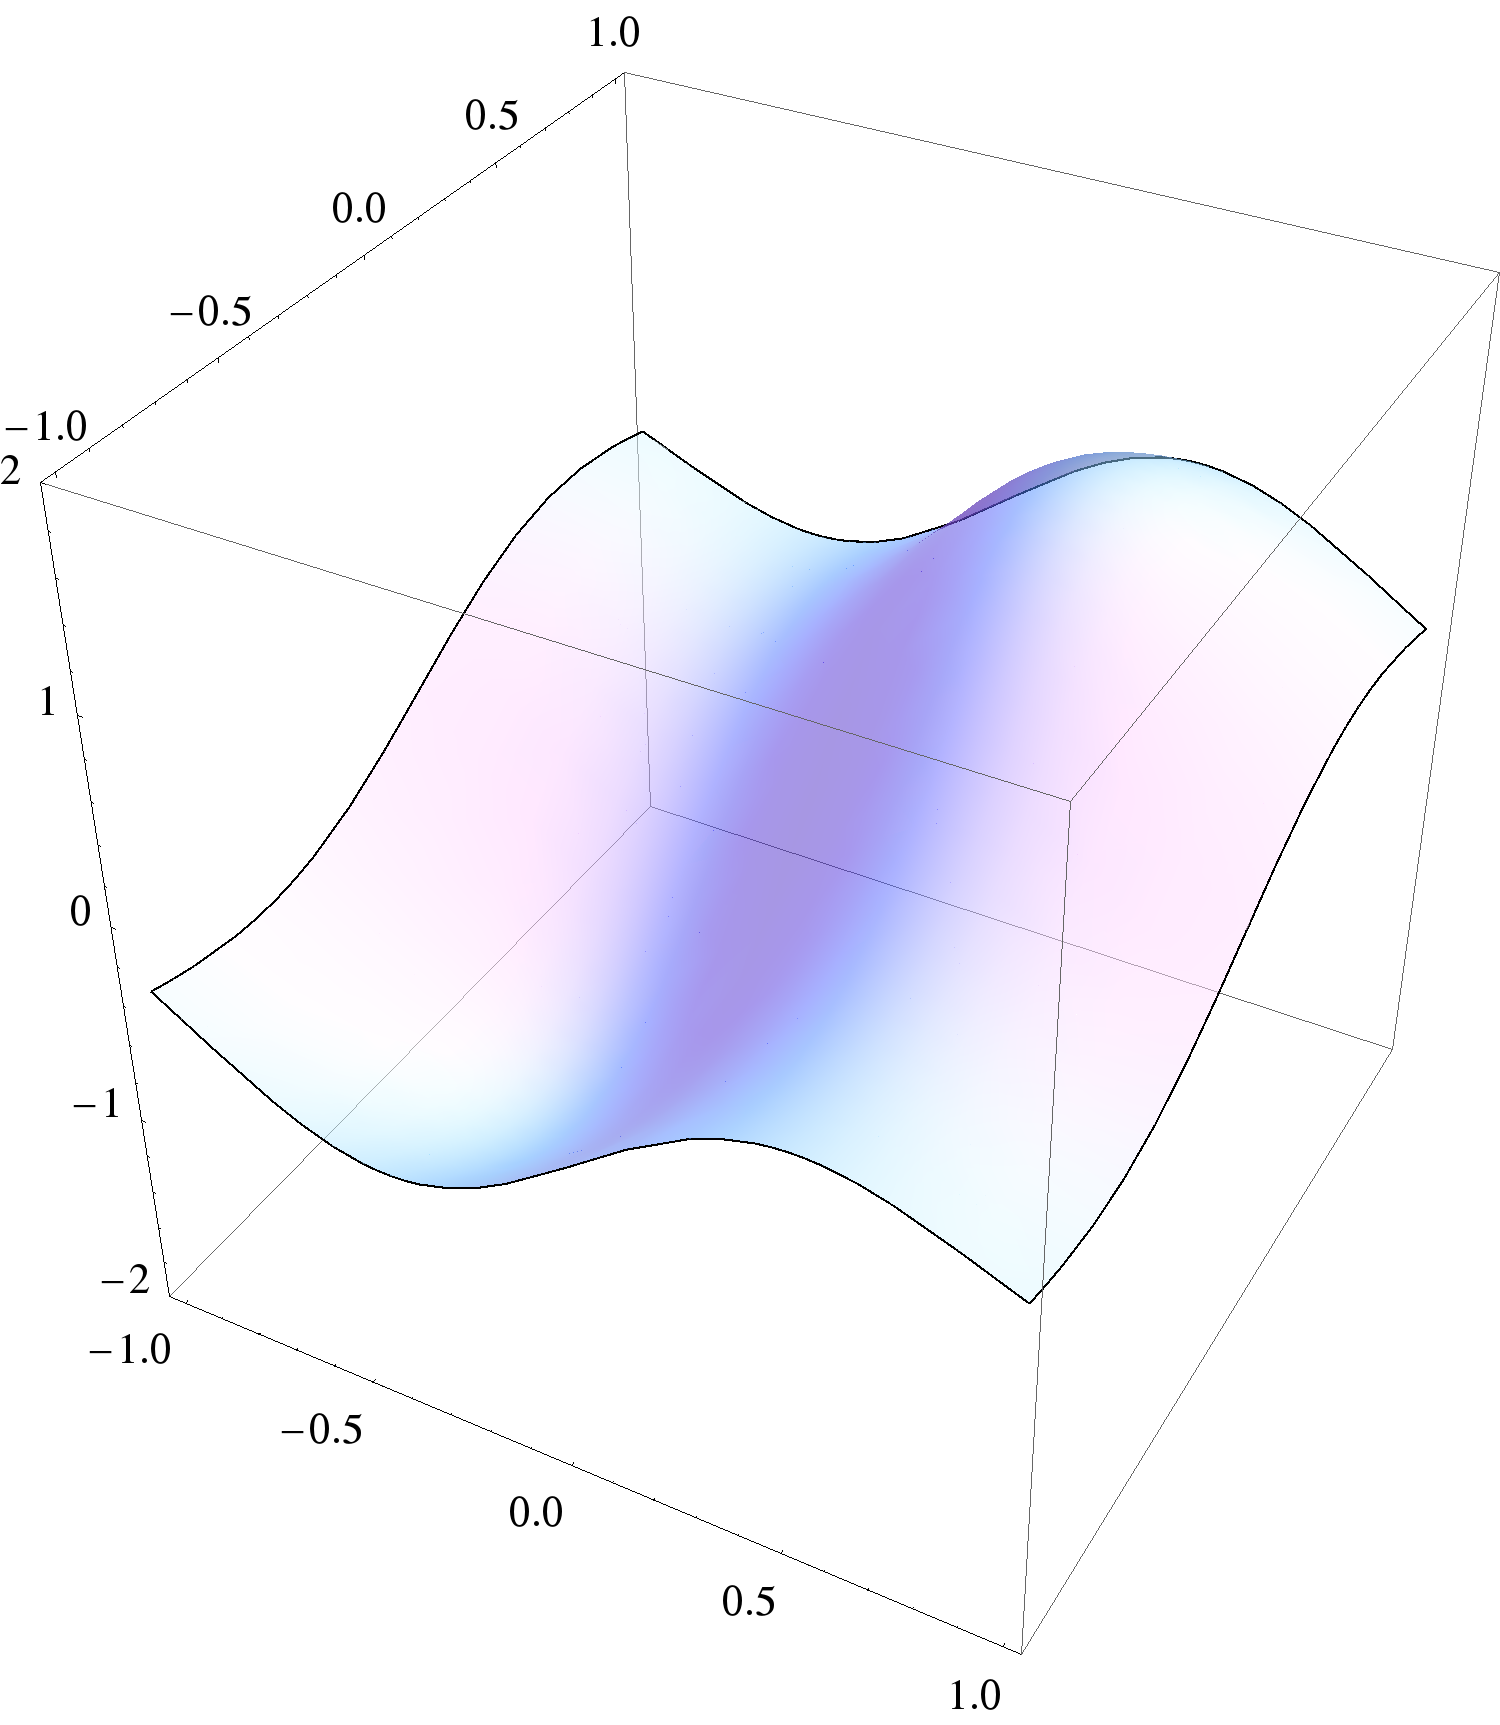
\includegraphics{surf1.png}
  \end{image}
  The gradient field of $F$ looks like this:
  \begin{image}
    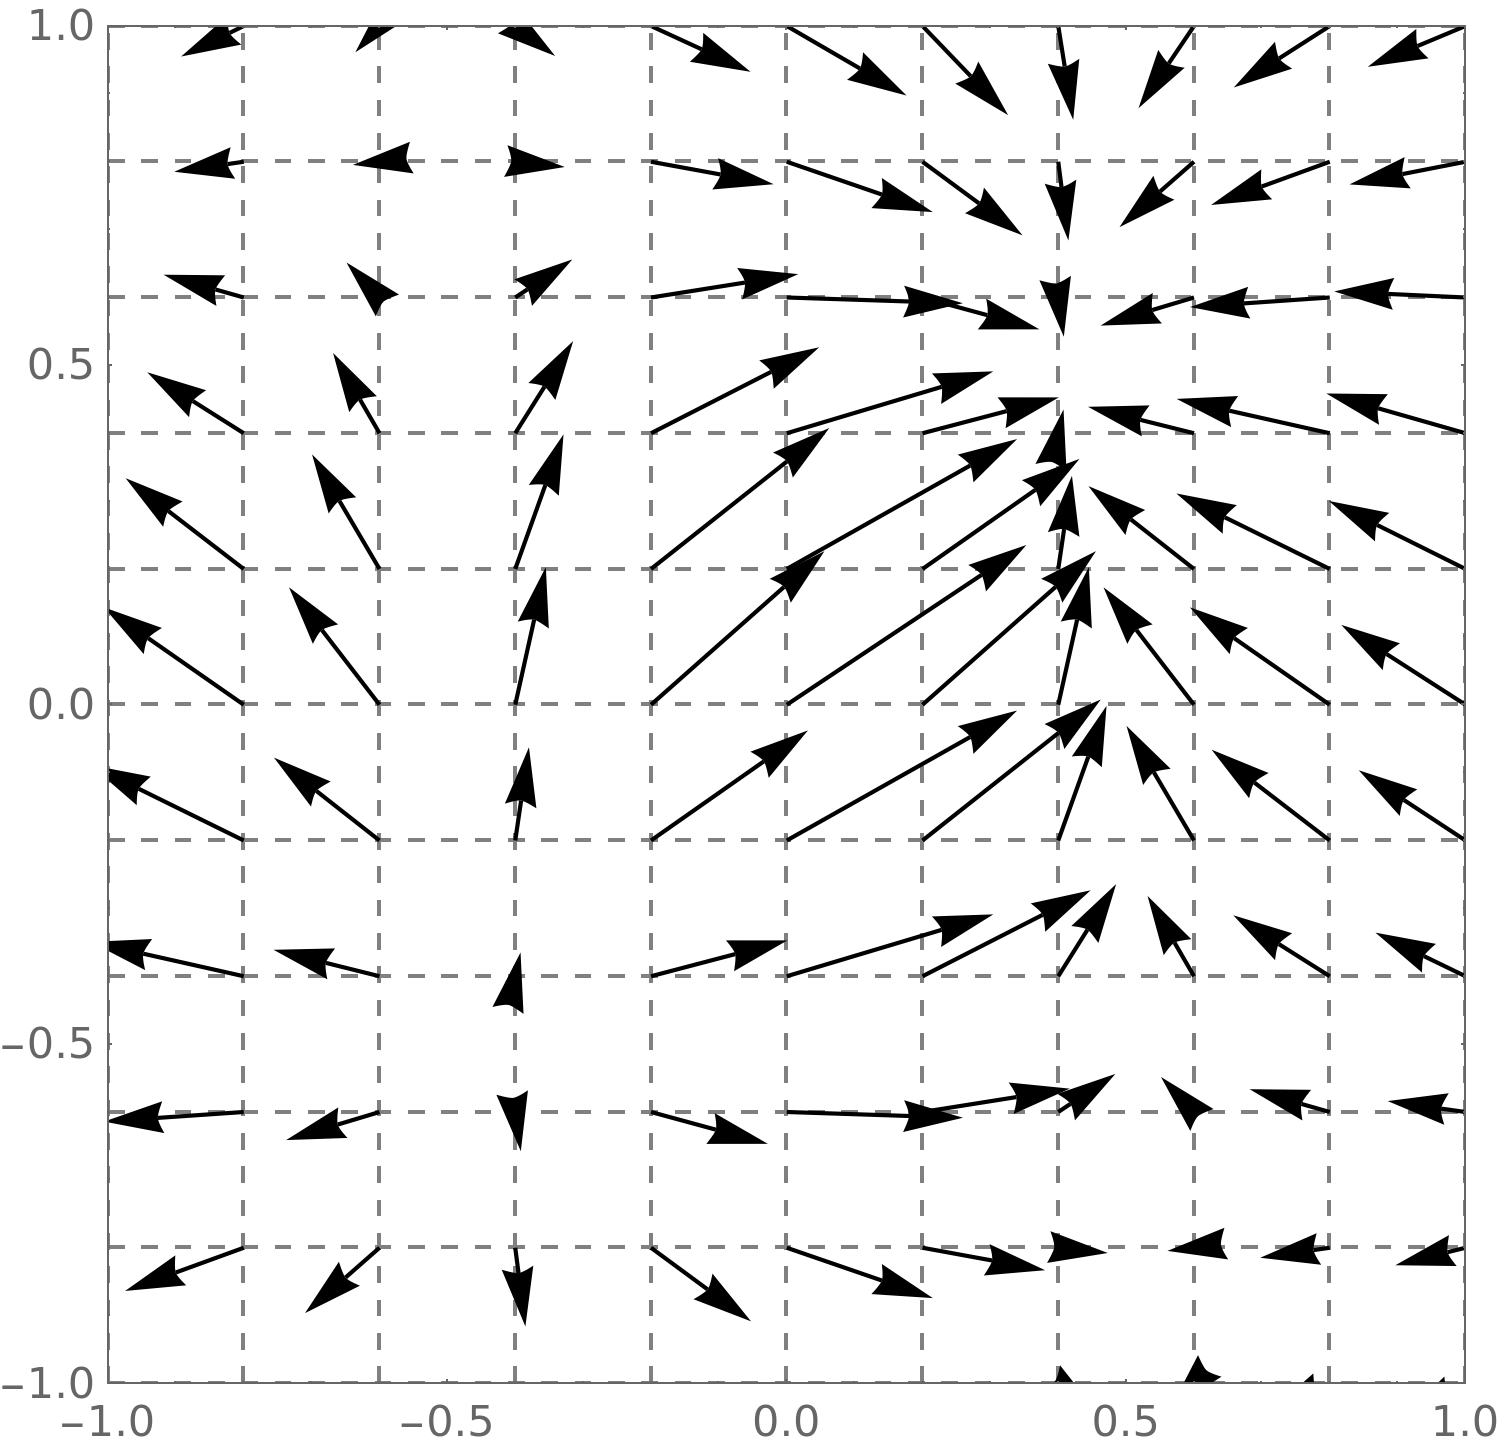
\includegraphics{gradField1.png}
  \end{image}
  Note we can see the vector pointing in the initial direction of
  greatest increase. Let's see a plot of both together:
  \begin{image}
    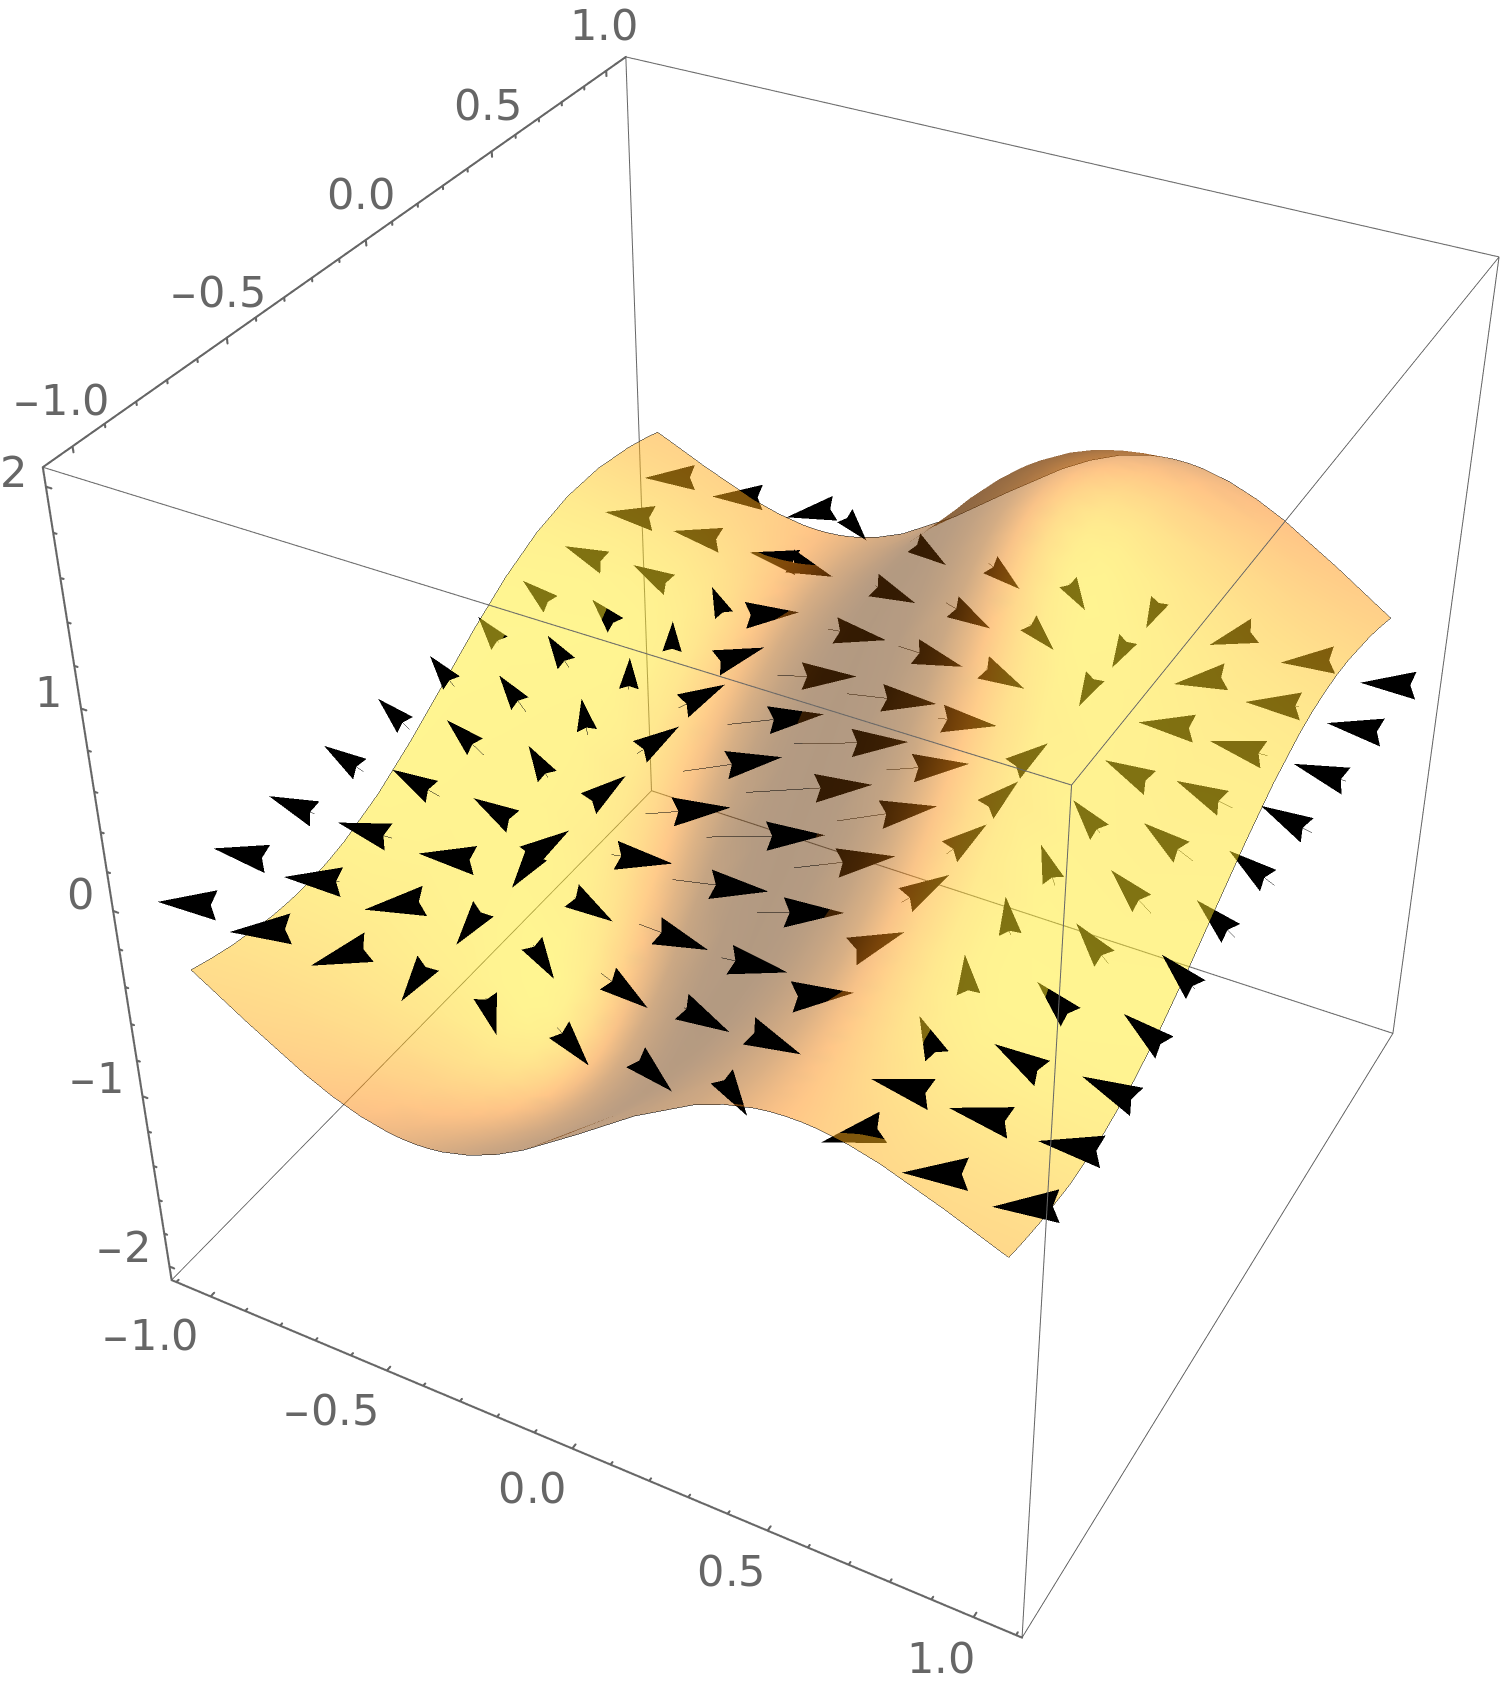
\includegraphics{gradSurf1.png}
  \end{image}
\end{example}

\begin{question}
  What is the connection between gradient vectors and level curves?
  \begin{prompt}
    \begin{multipleChoice}
      \choice[correct]{Gradient vectors are orthogonal to level curves.}
      \choice{Gradient vectors point in the direction of level curves.}
      \choice{Gradient vectors are independent of level curves.}
    \end{multipleChoice}
  \end{prompt}
\end{question}

\begin{example}
  Now consider $F(x,y) = \frac{1}{\sqrt{x^2+y^2}}$. A plot of this
    function looks like this:
  \[
  \vec{F}(x,y) = \vector{\frac{-x}{(x^2+y^2)^{3/2}},\frac{-y}{(x^2+y^2)^{3/2}}}:
  \]
  \begin{image}
    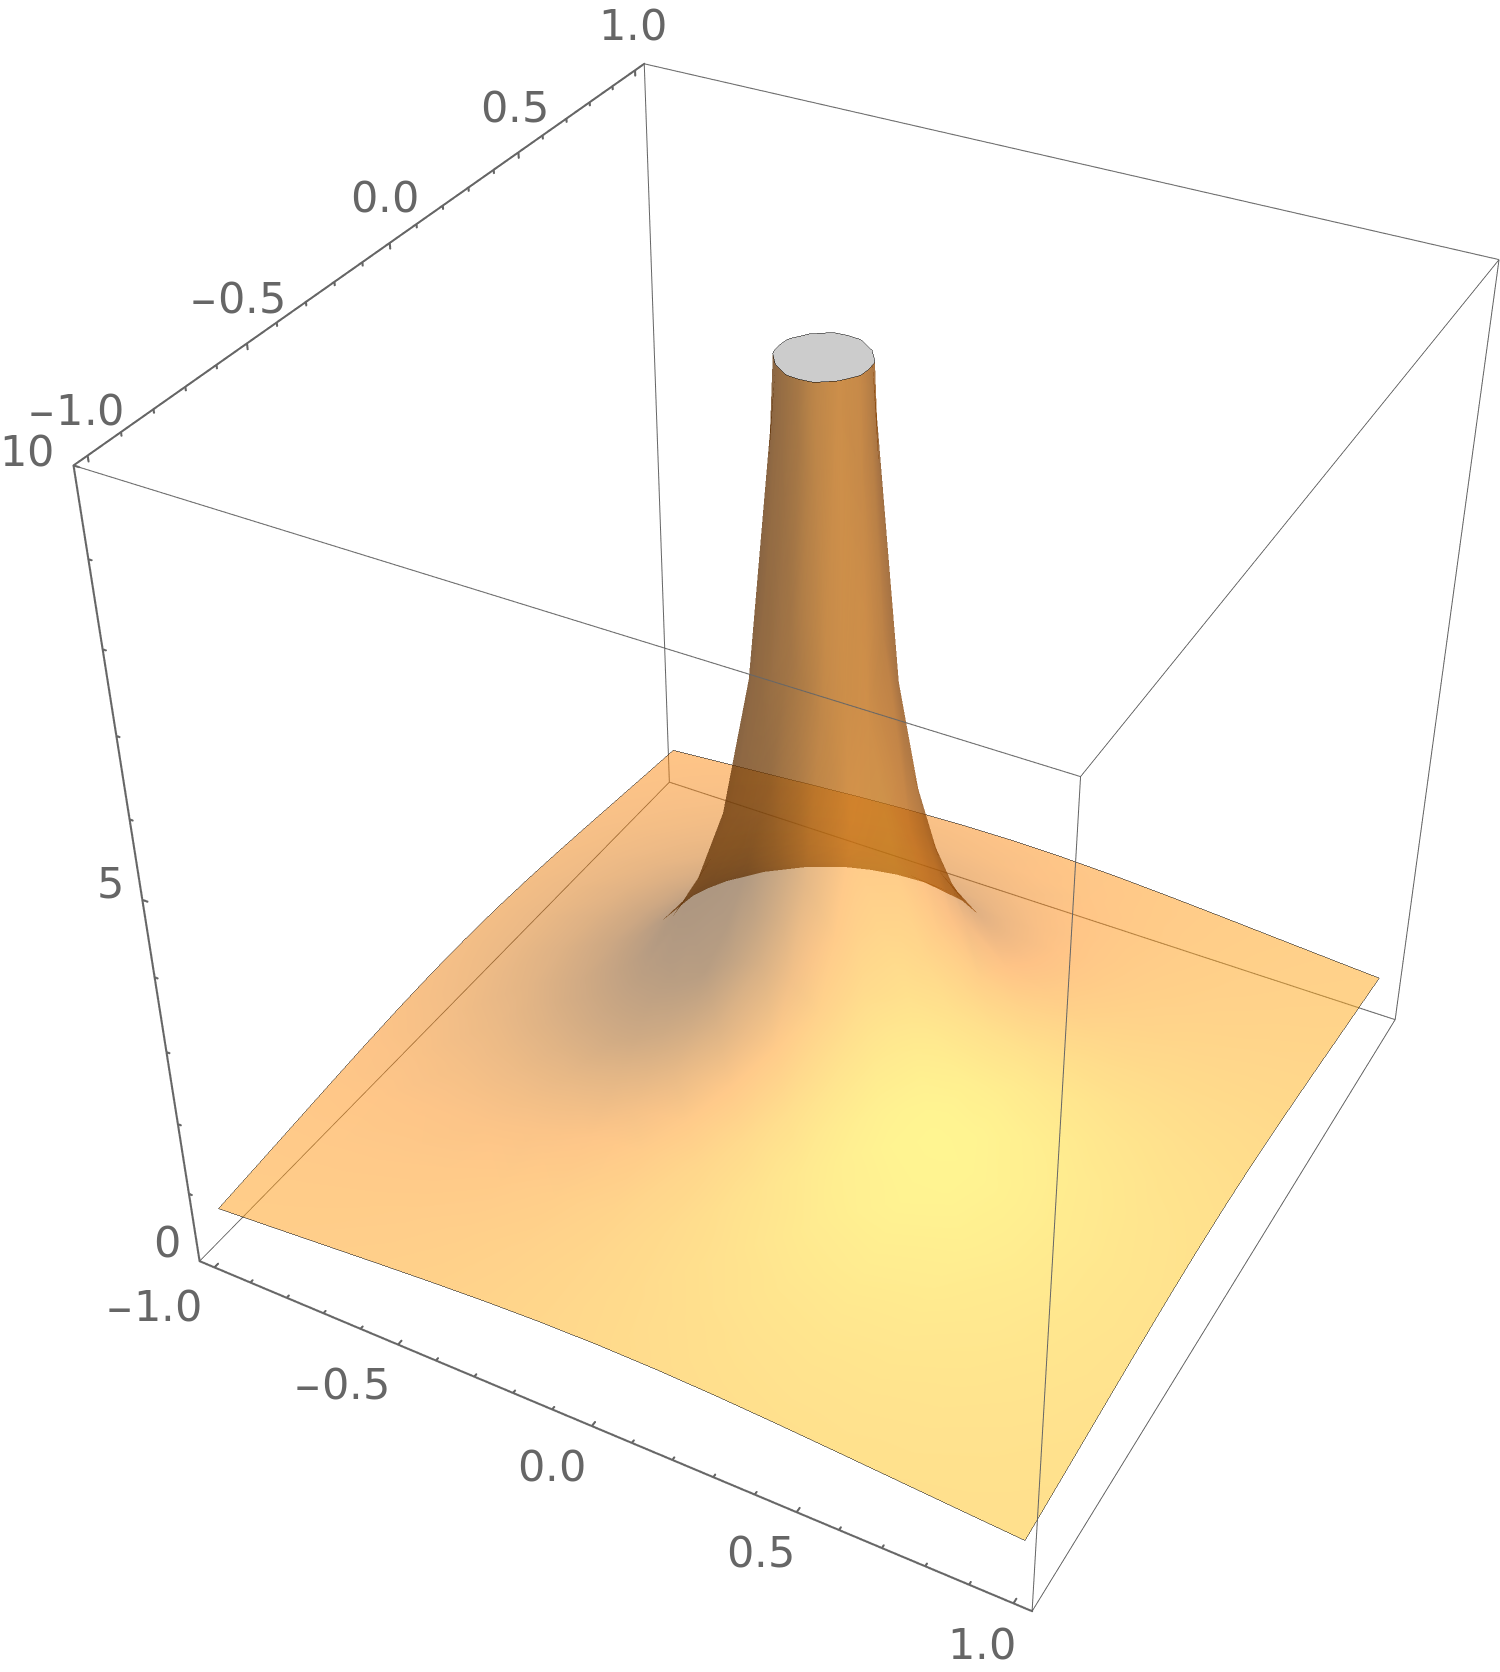
\includegraphics{surf2.png}
  \end{image}
  The gradient field of $F$ looks like this:
  \begin{image}
    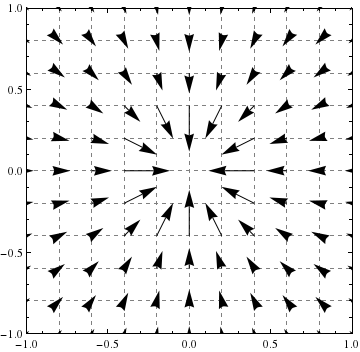
\includegraphics{gradField2.png}
  \end{image}
  Note we can see the vector pointing in the initial direction of
  greatest increase. Let's see a plot of both together:
  \begin{image}
    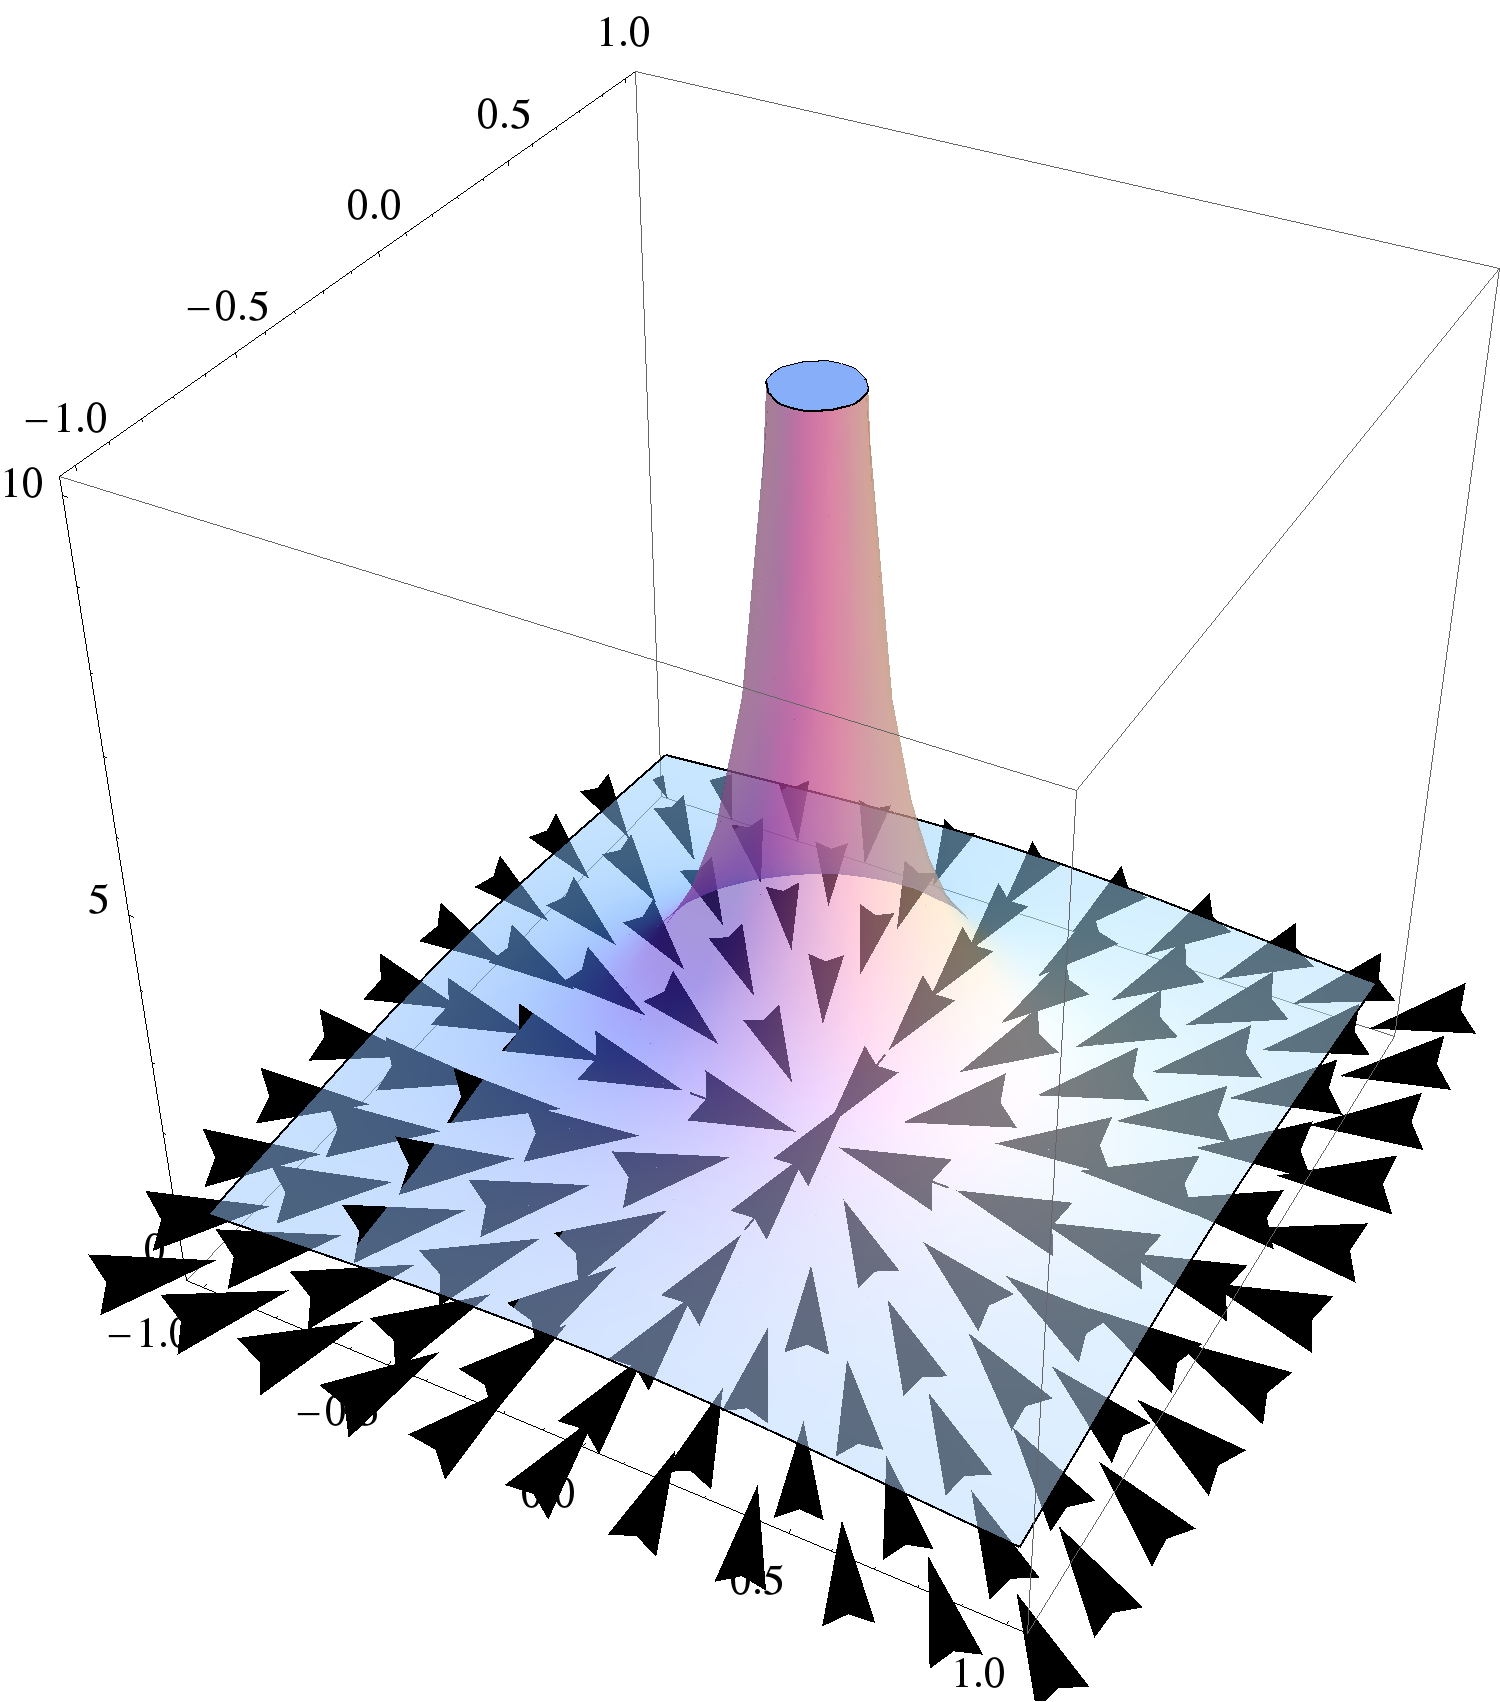
\includegraphics{gradSurf2.png}
  \end{image}
\end{example}




\subsection{The Clairaut gradient test} 

Now we give a method to determine if a field is a gradient field. 

\begin{theorem}[Clairaut]
  A vector field $\vec{F}(x,y) = \vector{M(x,y),N(x,y)}$, where $M$ and
  $N$ have continuous partial derivatives, is a gradient field if and
  only if
  \[
  \pp[N]{x} -\pp[M]{y} = \vec{0}  
  \]
  for all $x$ and $y$.
\end{theorem}


\begin{definition}
  If $\vec{G} = \grad F$, then $F$ is called a \dfn{potential
    function} for $\vec{G}$.
\end{definition}

\begin{question}
  Is $\vec{G} = \vector{2x+y^2,2y+x^2}$ a gradient field?
  \begin{multipleChoice}
    \choice{yes}
    \choice[correct]{no}
  \end{multipleChoice}
\end{question}


\begin{question}
  Is $\vec{G} = \vector{x^3,-y^4}$ a gradient field?
  \begin{multipleChoice}
    \choice[correct]{yes}
    \choice{no}
  \end{multipleChoice}
  \begin{question}
    Find a potential function $F$ such that $F(\vec{0}) = 0$.
    \begin{prompt}
      \[
      F(x,y) = \answer{x^4/4-y^5/5}.
      \]
    \end{prompt}
  \end{question}
\end{question}

\begin{question}
  Is $\vec{G} = \vector{y\cos(x),\sin(x)}$ a gradient field?
  \begin{multipleChoice}
    \choice[correct]{yes}
    \choice{no}
  \end{multipleChoice}
  \begin{question}
    Find a potential function $F$ such that $F(\vec{0}) = 0$.
    \begin{prompt}
      \[
      F(x,y) = \answer{y\sin(x)}.
      \]
    \end{prompt}
  \end{question}
\end{question}

\begin{question}
  Is $\vec{G} = \vector{\frac{-y}{x^2+y^2},\frac{x}{x^2+y^2}}$ a
  gradient field?
  \begin{multipleChoice}
    \choice{yes}
    \choice[correct]{no}
  \end{multipleChoice}
  \begin{feedback}
    What happens at $\vec{0}$?
  \end{feedback}
\end{question}

\end{document}
